% figures/fig5_captions.tex
% Generated by src/analysis/make_ch5_figures.py on 2026-09-11.
% Every number below was computed by that script from the same arrays it
% plotted; do not edit them by hand. CR data SHA-8 710f4a24
% (L_grid sha256 2d92b58e1693107d...).
%
% Usage:  % figures/fig5_captions.tex
% Generated by src/analysis/make_ch5_figures.py on 2026-09-11.
% Every number below was computed by that script from the same arrays it
% plotted; do not edit them by hand. CR data SHA-8 710f4a24
% (L_grid sha256 2d92b58e1693107d...).
%
% Usage:  % figures/fig5_captions.tex
% Generated by src/analysis/make_ch5_figures.py on 2026-09-11.
% Every number below was computed by that script from the same arrays it
% plotted; do not edit them by hand. CR data SHA-8 710f4a24
% (L_grid sha256 2d92b58e1693107d...).
%
% Usage:  % figures/fig5_captions.tex
% Generated by src/analysis/make_ch5_figures.py on 2026-09-11.
% Every number below was computed by that script from the same arrays it
% plotted; do not edit them by hand. CR data SHA-8 710f4a24
% (L_grid sha256 2d92b58e1693107d...).
%
% Usage:  \input{figures/fig5_captions.tex}  in the preamble, then
%   \begin{figure}[t]\centering
%     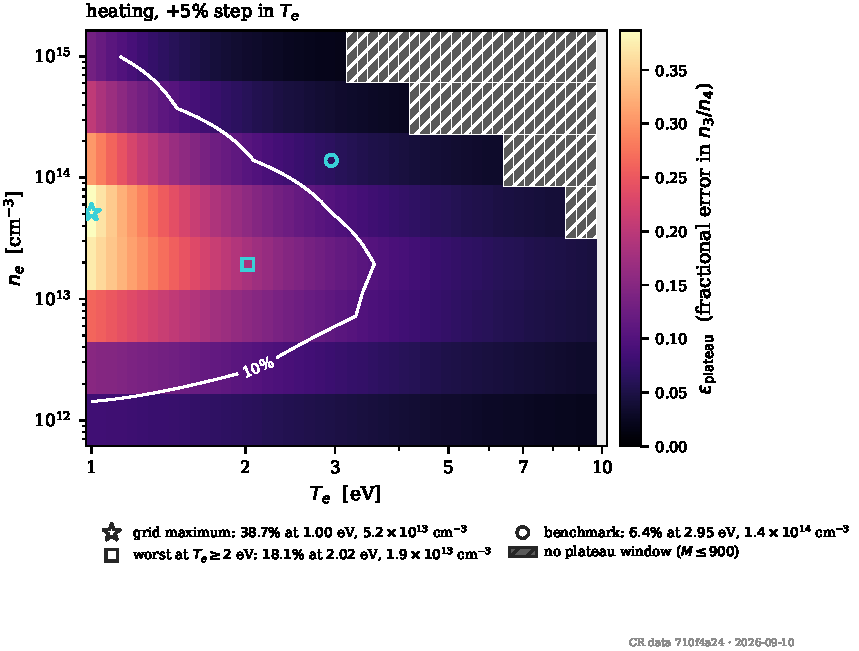
\includegraphics{figures/fig5_1_eps_map.pdf}
%     \caption{\CapFigEpsMap}\label{fig:eps-map}
%   \end{figure}

\newcommand{\CapFigEpsMap}{%
  \textbf{Where the quasi-steady-state closure fails.}
  Fractional error $\varepsilon_{\rm plateau}$ in the $n=3/n=4$ shell
  population ratio committed while the excited manifold has reached partial
  equilibrium but the ground state has not yet responded, after a
  $+5\%$ step in $T_e$ at fixed $n_e$ --- the \emph{heating} direction.
  Cooling is not the mirror image: the same transition between the two
  coldest grid temperatures, at $n_e = 1.9\times10^{13}$~cm$^{-3}$, gives 37.1\%
  heated and 28.6\% cooled, and the grid maximum moves from
  $[0,4]$ ($1.00$~eV, $5.2\times10^{13}$~cm$^{-3}$) to
  $[1,3]$ ($1.05$~eV, $1.9\times10^{13}$~cm$^{-3}$),
  where it is 28.6\%.
  Hatched cells have no timescale-separated plateau window
  ($M \leq 900$, 54 of the heated cells): a plateau value is not
  defined there and none is plotted. The plain grey strip at the right-hand
  edge is the hottest temperature row, from which a $+5\%$ step cannot
  reach a new grid index. The three marked cells, keyed below the axes, are
  the grid maximum (38.7\% at $T_e = 1.00$~eV,
  $n_e = 5.2\times10^{13}$~cm$^{-3}$), the largest value at $T_e \geq 2$~eV
  (18.1\% at $T_e = 2.02$~eV, $n_e = 1.9\times10^{13}$~cm$^{-3}$), and the
  thesis benchmark point ($T_e = 2.947$~eV,
  $n_e = 1.39\times10^{14}$~cm$^{-3}$, 6.36\%).
  Below $2$~eV the values shown are upper estimates: switching on Lyman
  trapping divides the grid maximum by $2.5$--$3.3$ depending on the assumed
  slab thickness, and below $1.15$~eV it also moves which density column
  carries the maximum (Figure~\ref{fig:trapping}). Nothing on the cold edge of
  this map is quantitative.}

\newcommand{\CapFigEpsVsNe}{%
  \textbf{The density dependence, all 8 columns.}
  $\varepsilon_{\rm plateau}$ against $n_e$ for 7 temperatures, heating,
  $+5\%$ step. Every density column computed is shown; stars mark each
  row's maximum, open symbols mark points with no plateau window.
  Each row has a single interior maximum, but it is
  \emph{broad and shallow in $\log n_e$}: across the peak column and its two
  neighbours --- a factor 7.2 in density --- $\varepsilon$ varies by
  only 6--22\%, so the location of the maximum is not
  resolved to better than about one grid interval, a factor 2.68. Over the
  full three decades the same row falls by a factor
  2.2--6.6: the structure is a real crest in density, but
  a wide-topped one, and the word ridge should not be read as implying a sharp
  or well-localised line. The column at $n_e = 5.2\times10^{13}$~cm$^{-3}$ carries the row
  maximum in 3 of 49 heating rows, all of them the coldest; at every
  warmer temperature the maximum sits at $1.9\times10^{13}$~cm$^{-3}$. Both columns must
  be reported: quoting either alone misstates where the closure is worst, and
  below $1.15$~eV the position moves across three columns once Lyman trapping
  is included (Figure~\ref{fig:trapping}), so no maximum location is claimed
  there at all.}

\newcommand{\CapFigMvsEps}{%
  \textbf{Timescale separation does not predict closure error.}
  Each point is one (grid point, step direction) pair with a
  timescale-separated plateau window (680 of 784); $M$ is
  $\tau_{\rm slow}/\tau_{\rm relax}$ of the post-step operator, colour is $T_e$,
  circles heating and triangles cooling. The raw association is strong,
  $\mathrm{corr}(\log M, \log\varepsilon) = +0.76$, and it is a temperature
  proxy rather than a dynamical statement: $\log M$ is 93\% explained by
  $(\log T_e, \log n_e)$ alone, a bare Arrhenius factor $e^{13.6/T_e}$
  containing no dynamics correlates at +0.71, and controlling for
  $(\log T_e, \log n_e)$ drives the association to +0.27 linearly and
  -0.44 --- the opposite sign --- quadratically. The two starred extrema make
  the same point without statistics: the largest $M$ on the grid
  ($1.7\times10^{9}$, blue) carries $\varepsilon = 12.0\%$, while the largest
  error (38.7\%, red) occurs 52$\times$ away in density, at an $M$
  smaller by a factor 46. A large timescale separation is not evidence that
  the quasi-steady-state closure is accurate.}

\newcommand{\CapFigTrapping}{%
  \textbf{Lyman trapping, and why the quantitative scope starts at 2~eV.}
  (a) $\varepsilon_{\rm plateau}$ against the assumed homogeneous-slab
  thickness $D$ used for the Lyman escape factors, computed self-consistently
  ($\Theta_P$ depends on $n(1s)$, which depends on $\Theta_P$) for all 14
  Lyman channels; $D = 0$ is the optically thin matrix used everywhere else in
  this chapter. The grid maximum at $T_e = 1.00$~eV falls from
  38.7\% to 11.6--15.7\% over $D = 1$--20~cm: the cold-edge
  number is set by a slab thickness this zero-dimensional model does not
  contain, and must never be quoted without it. The worst point at
  $T_e \geq 2$~eV moves by 0.5\% and the benchmark by 0.7\%
  over the same twentyfold range. (b) Number of analysed pairs exceeding the
  $10\%$ threshold, counted on the plateau value itself and not on the
  time-averaged ELM bound: 225 falls to 177 over the whole map, while
  above $2$~eV it is 63 against 62 --- unchanged to within one
  pair. (At $D = 20$~cm the analysed set is 678 pairs rather than
  680: two lose their plateau window.)
  The $T_e \geq 2$~eV restriction is therefore not a hedge; it is the measured
  boundary beyond which the one neglected process most likely to invalidate
  the result stops mattering.}
  in the preamble, then
%   \begin{figure}[t]\centering
%     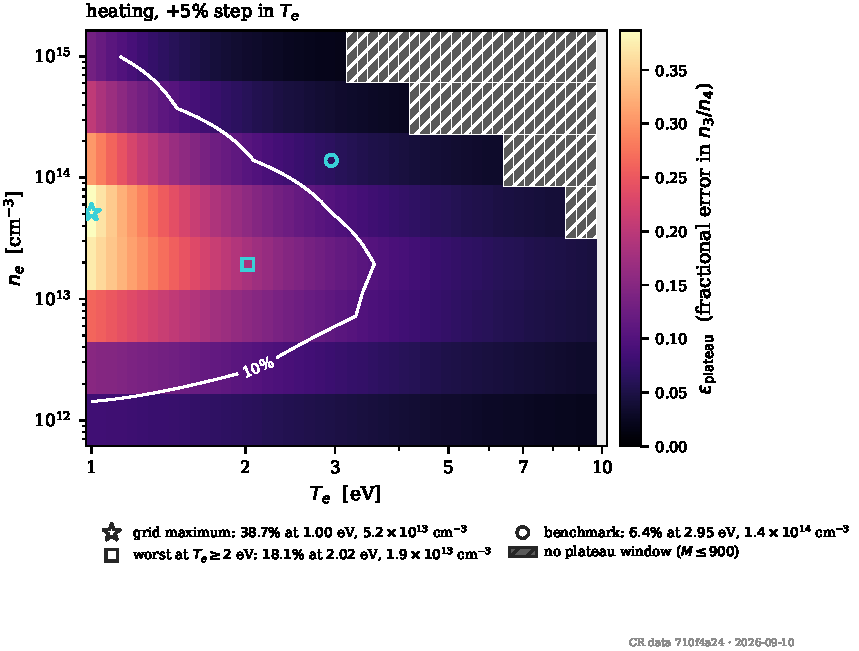
\includegraphics{figures/fig5_1_eps_map.pdf}
%     \caption{\CapFigEpsMap}\label{fig:eps-map}
%   \end{figure}

\newcommand{\CapFigEpsMap}{%
  \textbf{Where the quasi-steady-state closure fails.}
  Fractional error $\varepsilon_{\rm plateau}$ in the $n=3/n=4$ shell
  population ratio committed while the excited manifold has reached partial
  equilibrium but the ground state has not yet responded, after a
  $+5\%$ step in $T_e$ at fixed $n_e$ --- the \emph{heating} direction.
  Cooling is not the mirror image: the same transition between the two
  coldest grid temperatures, at $n_e = 1.9\times10^{13}$~cm$^{-3}$, gives 37.1\%
  heated and 28.6\% cooled, and the grid maximum moves from
  $[0,4]$ ($1.00$~eV, $5.2\times10^{13}$~cm$^{-3}$) to
  $[1,3]$ ($1.05$~eV, $1.9\times10^{13}$~cm$^{-3}$),
  where it is 28.6\%.
  Hatched cells have no timescale-separated plateau window
  ($M \leq 900$, 54 of the heated cells): a plateau value is not
  defined there and none is plotted. The plain grey strip at the right-hand
  edge is the hottest temperature row, from which a $+5\%$ step cannot
  reach a new grid index. The three marked cells, keyed below the axes, are
  the grid maximum (38.7\% at $T_e = 1.00$~eV,
  $n_e = 5.2\times10^{13}$~cm$^{-3}$), the largest value at $T_e \geq 2$~eV
  (18.1\% at $T_e = 2.02$~eV, $n_e = 1.9\times10^{13}$~cm$^{-3}$), and the
  thesis benchmark point ($T_e = 2.947$~eV,
  $n_e = 1.39\times10^{14}$~cm$^{-3}$, 6.36\%).
  Below $2$~eV the values shown are upper estimates: switching on Lyman
  trapping divides the grid maximum by $2.5$--$3.3$ depending on the assumed
  slab thickness, and below $1.15$~eV it also moves which density column
  carries the maximum (Figure~\ref{fig:trapping}). Nothing on the cold edge of
  this map is quantitative.}

\newcommand{\CapFigEpsVsNe}{%
  \textbf{The density dependence, all 8 columns.}
  $\varepsilon_{\rm plateau}$ against $n_e$ for 7 temperatures, heating,
  $+5\%$ step. Every density column computed is shown; stars mark each
  row's maximum, open symbols mark points with no plateau window.
  Each row has a single interior maximum, but it is
  \emph{broad and shallow in $\log n_e$}: across the peak column and its two
  neighbours --- a factor 7.2 in density --- $\varepsilon$ varies by
  only 6--22\%, so the location of the maximum is not
  resolved to better than about one grid interval, a factor 2.68. Over the
  full three decades the same row falls by a factor
  2.2--6.6: the structure is a real crest in density, but
  a wide-topped one, and the word ridge should not be read as implying a sharp
  or well-localised line. The column at $n_e = 5.2\times10^{13}$~cm$^{-3}$ carries the row
  maximum in 3 of 49 heating rows, all of them the coldest; at every
  warmer temperature the maximum sits at $1.9\times10^{13}$~cm$^{-3}$. Both columns must
  be reported: quoting either alone misstates where the closure is worst, and
  below $1.15$~eV the position moves across three columns once Lyman trapping
  is included (Figure~\ref{fig:trapping}), so no maximum location is claimed
  there at all.}

\newcommand{\CapFigMvsEps}{%
  \textbf{Timescale separation does not predict closure error.}
  Each point is one (grid point, step direction) pair with a
  timescale-separated plateau window (680 of 784); $M$ is
  $\tau_{\rm slow}/\tau_{\rm relax}$ of the post-step operator, colour is $T_e$,
  circles heating and triangles cooling. The raw association is strong,
  $\mathrm{corr}(\log M, \log\varepsilon) = +0.76$, and it is a temperature
  proxy rather than a dynamical statement: $\log M$ is 93\% explained by
  $(\log T_e, \log n_e)$ alone, a bare Arrhenius factor $e^{13.6/T_e}$
  containing no dynamics correlates at +0.71, and controlling for
  $(\log T_e, \log n_e)$ drives the association to +0.27 linearly and
  -0.44 --- the opposite sign --- quadratically. The two starred extrema make
  the same point without statistics: the largest $M$ on the grid
  ($1.7\times10^{9}$, blue) carries $\varepsilon = 12.0\%$, while the largest
  error (38.7\%, red) occurs 52$\times$ away in density, at an $M$
  smaller by a factor 46. A large timescale separation is not evidence that
  the quasi-steady-state closure is accurate.}

\newcommand{\CapFigTrapping}{%
  \textbf{Lyman trapping, and why the quantitative scope starts at 2~eV.}
  (a) $\varepsilon_{\rm plateau}$ against the assumed homogeneous-slab
  thickness $D$ used for the Lyman escape factors, computed self-consistently
  ($\Theta_P$ depends on $n(1s)$, which depends on $\Theta_P$) for all 14
  Lyman channels; $D = 0$ is the optically thin matrix used everywhere else in
  this chapter. The grid maximum at $T_e = 1.00$~eV falls from
  38.7\% to 11.6--15.7\% over $D = 1$--20~cm: the cold-edge
  number is set by a slab thickness this zero-dimensional model does not
  contain, and must never be quoted without it. The worst point at
  $T_e \geq 2$~eV moves by 0.5\% and the benchmark by 0.7\%
  over the same twentyfold range. (b) Number of analysed pairs exceeding the
  $10\%$ threshold, counted on the plateau value itself and not on the
  time-averaged ELM bound: 225 falls to 177 over the whole map, while
  above $2$~eV it is 63 against 62 --- unchanged to within one
  pair. (At $D = 20$~cm the analysed set is 678 pairs rather than
  680: two lose their plateau window.)
  The $T_e \geq 2$~eV restriction is therefore not a hedge; it is the measured
  boundary beyond which the one neglected process most likely to invalidate
  the result stops mattering.}
  in the preamble, then
%   \begin{figure}[t]\centering
%     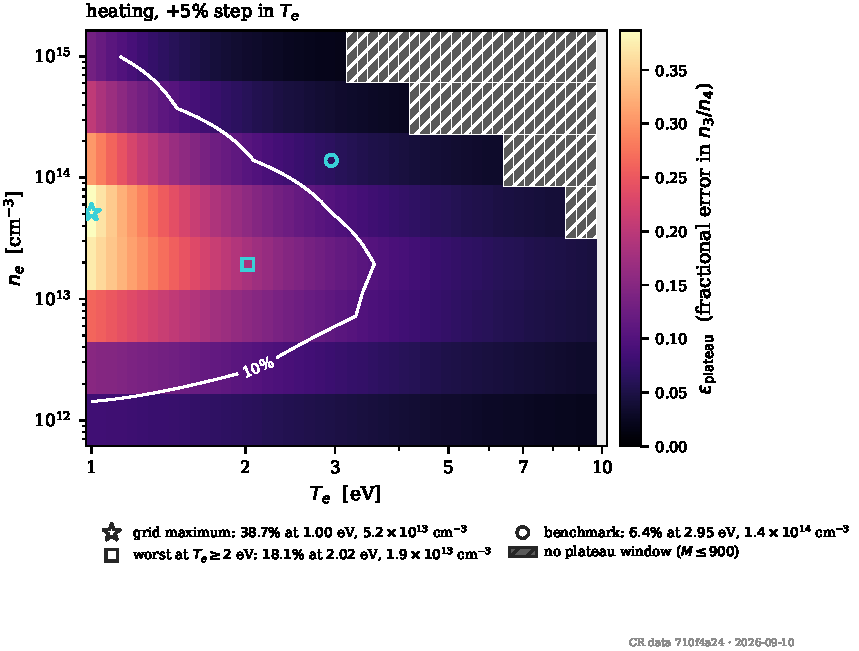
\includegraphics{figures/fig5_1_eps_map.pdf}
%     \caption{\CapFigEpsMap}\label{fig:eps-map}
%   \end{figure}

\newcommand{\CapFigEpsMap}{%
  \textbf{Where the quasi-steady-state closure fails.}
  Fractional error $\varepsilon_{\rm plateau}$ in the $n=3/n=4$ shell
  population ratio committed while the excited manifold has reached partial
  equilibrium but the ground state has not yet responded, after a
  $+5\%$ step in $T_e$ at fixed $n_e$ --- the \emph{heating} direction.
  Cooling is not the mirror image: the same transition between the two
  coldest grid temperatures, at $n_e = 1.9\times10^{13}$~cm$^{-3}$, gives 37.1\%
  heated and 28.6\% cooled, and the grid maximum moves from
  $[0,4]$ ($1.00$~eV, $5.2\times10^{13}$~cm$^{-3}$) to
  $[1,3]$ ($1.05$~eV, $1.9\times10^{13}$~cm$^{-3}$),
  where it is 28.6\%.
  Hatched cells have no timescale-separated plateau window
  ($M \leq 900$, 54 of the heated cells): a plateau value is not
  defined there and none is plotted. The plain grey strip at the right-hand
  edge is the hottest temperature row, from which a $+5\%$ step cannot
  reach a new grid index. The three marked cells, keyed below the axes, are
  the grid maximum (38.7\% at $T_e = 1.00$~eV,
  $n_e = 5.2\times10^{13}$~cm$^{-3}$), the largest value at $T_e \geq 2$~eV
  (18.1\% at $T_e = 2.02$~eV, $n_e = 1.9\times10^{13}$~cm$^{-3}$), and the
  thesis benchmark point ($T_e = 2.947$~eV,
  $n_e = 1.39\times10^{14}$~cm$^{-3}$, 6.36\%).
  Below $2$~eV the values shown are upper estimates: switching on Lyman
  trapping divides the grid maximum by $2.5$--$3.3$ depending on the assumed
  slab thickness, and below $1.15$~eV it also moves which density column
  carries the maximum (Figure~\ref{fig:trapping}). Nothing on the cold edge of
  this map is quantitative.}

\newcommand{\CapFigEpsVsNe}{%
  \textbf{The density dependence, all 8 columns.}
  $\varepsilon_{\rm plateau}$ against $n_e$ for 7 temperatures, heating,
  $+5\%$ step. Every density column computed is shown; stars mark each
  row's maximum, open symbols mark points with no plateau window.
  Each row has a single interior maximum, but it is
  \emph{broad and shallow in $\log n_e$}: across the peak column and its two
  neighbours --- a factor 7.2 in density --- $\varepsilon$ varies by
  only 6--22\%, so the location of the maximum is not
  resolved to better than about one grid interval, a factor 2.68. Over the
  full three decades the same row falls by a factor
  2.2--6.6: the structure is a real crest in density, but
  a wide-topped one, and the word ridge should not be read as implying a sharp
  or well-localised line. The column at $n_e = 5.2\times10^{13}$~cm$^{-3}$ carries the row
  maximum in 3 of 49 heating rows, all of them the coldest; at every
  warmer temperature the maximum sits at $1.9\times10^{13}$~cm$^{-3}$. Both columns must
  be reported: quoting either alone misstates where the closure is worst, and
  below $1.15$~eV the position moves across three columns once Lyman trapping
  is included (Figure~\ref{fig:trapping}), so no maximum location is claimed
  there at all.}

\newcommand{\CapFigMvsEps}{%
  \textbf{Timescale separation does not predict closure error.}
  Each point is one (grid point, step direction) pair with a
  timescale-separated plateau window (680 of 784); $M$ is
  $\tau_{\rm slow}/\tau_{\rm relax}$ of the post-step operator, colour is $T_e$,
  circles heating and triangles cooling. The raw association is strong,
  $\mathrm{corr}(\log M, \log\varepsilon) = +0.76$, and it is a temperature
  proxy rather than a dynamical statement: $\log M$ is 93\% explained by
  $(\log T_e, \log n_e)$ alone, a bare Arrhenius factor $e^{13.6/T_e}$
  containing no dynamics correlates at +0.71, and controlling for
  $(\log T_e, \log n_e)$ drives the association to +0.27 linearly and
  -0.44 --- the opposite sign --- quadratically. The two starred extrema make
  the same point without statistics: the largest $M$ on the grid
  ($1.7\times10^{9}$, blue) carries $\varepsilon = 12.0\%$, while the largest
  error (38.7\%, red) occurs 52$\times$ away in density, at an $M$
  smaller by a factor 46. A large timescale separation is not evidence that
  the quasi-steady-state closure is accurate.}

\newcommand{\CapFigTrapping}{%
  \textbf{Lyman trapping, and why the quantitative scope starts at 2~eV.}
  (a) $\varepsilon_{\rm plateau}$ against the assumed homogeneous-slab
  thickness $D$ used for the Lyman escape factors, computed self-consistently
  ($\Theta_P$ depends on $n(1s)$, which depends on $\Theta_P$) for all 14
  Lyman channels; $D = 0$ is the optically thin matrix used everywhere else in
  this chapter. The grid maximum at $T_e = 1.00$~eV falls from
  38.7\% to 11.6--15.7\% over $D = 1$--20~cm: the cold-edge
  number is set by a slab thickness this zero-dimensional model does not
  contain, and must never be quoted without it. The worst point at
  $T_e \geq 2$~eV moves by 0.5\% and the benchmark by 0.7\%
  over the same twentyfold range. (b) Number of analysed pairs exceeding the
  $10\%$ threshold, counted on the plateau value itself and not on the
  time-averaged ELM bound: 225 falls to 177 over the whole map, while
  above $2$~eV it is 63 against 62 --- unchanged to within one
  pair. (At $D = 20$~cm the analysed set is 678 pairs rather than
  680: two lose their plateau window.)
  The $T_e \geq 2$~eV restriction is therefore not a hedge; it is the measured
  boundary beyond which the one neglected process most likely to invalidate
  the result stops mattering.}
  in the preamble, then
%   \begin{figure}[t]\centering
%     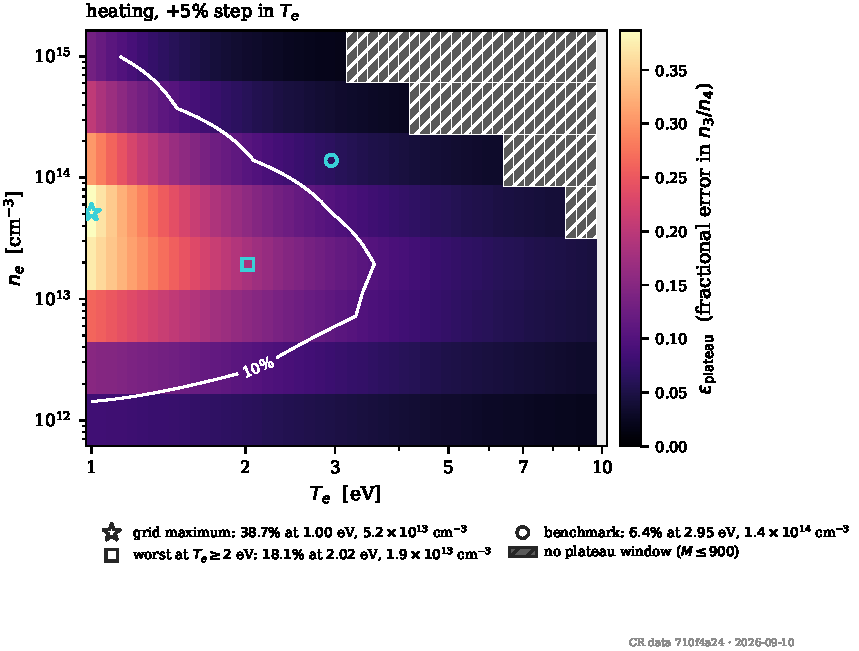
\includegraphics{figures/fig5_1_eps_map.pdf}
%     \caption{\CapFigEpsMap}\label{fig:eps-map}
%   \end{figure}

\newcommand{\CapFigEpsMap}{%
  \textbf{Where the quasi-steady-state closure fails.}
  Fractional error $\varepsilon_{\rm plateau}$ in the $n=3/n=4$ shell
  population ratio committed while the excited manifold has reached partial
  equilibrium but the ground state has not yet responded, after a
  $+5\%$ step in $T_e$ at fixed $n_e$ --- the \emph{heating} direction.
  Cooling is not the mirror image: the same transition between the two
  coldest grid temperatures, at $n_e = 1.9\times10^{13}$~cm$^{-3}$, gives 37.1\%
  heated and 28.6\% cooled, and the grid maximum moves from
  $[0,4]$ ($1.00$~eV, $5.2\times10^{13}$~cm$^{-3}$) to
  $[1,3]$ ($1.05$~eV, $1.9\times10^{13}$~cm$^{-3}$),
  where it is 28.6\%.
  Hatched cells have no timescale-separated plateau window
  ($M \leq 900$, 54 of the heated cells): a plateau value is not
  defined there and none is plotted. The plain grey strip at the right-hand
  edge is the hottest temperature row, from which a $+5\%$ step cannot
  reach a new grid index. The three marked cells, keyed below the axes, are
  the grid maximum (38.7\% at $T_e = 1.00$~eV,
  $n_e = 5.2\times10^{13}$~cm$^{-3}$), the largest value at $T_e \geq 2$~eV
  (18.1\% at $T_e = 2.02$~eV, $n_e = 1.9\times10^{13}$~cm$^{-3}$), and the
  thesis benchmark point ($T_e = 2.947$~eV,
  $n_e = 1.39\times10^{14}$~cm$^{-3}$, 6.36\%).
  Below $2$~eV the values shown are upper estimates: switching on Lyman
  trapping divides the grid maximum by $2.5$--$3.3$ depending on the assumed
  slab thickness, and below $1.15$~eV it also moves which density column
  carries the maximum (Figure~\ref{fig:trapping}). Nothing on the cold edge of
  this map is quantitative.}

\newcommand{\CapFigEpsVsNe}{%
  \textbf{The density dependence, all 8 columns.}
  $\varepsilon_{\rm plateau}$ against $n_e$ for 7 temperatures, heating,
  $+5\%$ step. Every density column computed is shown; stars mark each
  row's maximum, open symbols mark points with no plateau window.
  Each row has a single interior maximum, but it is
  \emph{broad and shallow in $\log n_e$}: across the peak column and its two
  neighbours --- a factor 7.2 in density --- $\varepsilon$ varies by
  only 6--22\%, so the location of the maximum is not
  resolved to better than about one grid interval, a factor 2.68. Over the
  full three decades the same row falls by a factor
  2.2--6.6: the structure is a real crest in density, but
  a wide-topped one, and the word ridge should not be read as implying a sharp
  or well-localised line. The column at $n_e = 5.2\times10^{13}$~cm$^{-3}$ carries the row
  maximum in 3 of 49 heating rows, all of them the coldest; at every
  warmer temperature the maximum sits at $1.9\times10^{13}$~cm$^{-3}$. Both columns must
  be reported: quoting either alone misstates where the closure is worst, and
  below $1.15$~eV the position moves across three columns once Lyman trapping
  is included (Figure~\ref{fig:trapping}), so no maximum location is claimed
  there at all.}

\newcommand{\CapFigMvsEps}{%
  \textbf{Timescale separation does not predict closure error.}
  Each point is one (grid point, step direction) pair with a
  timescale-separated plateau window (680 of 784); $M$ is
  $\tau_{\rm slow}/\tau_{\rm relax}$ of the post-step operator, colour is $T_e$,
  circles heating and triangles cooling. The raw association is strong,
  $\mathrm{corr}(\log M, \log\varepsilon) = +0.76$, and it is a temperature
  proxy rather than a dynamical statement: $\log M$ is 93\% explained by
  $(\log T_e, \log n_e)$ alone, a bare Arrhenius factor $e^{13.6/T_e}$
  containing no dynamics correlates at +0.71, and controlling for
  $(\log T_e, \log n_e)$ drives the association to +0.27 linearly and
  -0.44 --- the opposite sign --- quadratically. The two starred extrema make
  the same point without statistics: the largest $M$ on the grid
  ($1.7\times10^{9}$, blue) carries $\varepsilon = 12.0\%$, while the largest
  error (38.7\%, red) occurs 52$\times$ away in density, at an $M$
  smaller by a factor 46. A large timescale separation is not evidence that
  the quasi-steady-state closure is accurate.}

\newcommand{\CapFigTrapping}{%
  \textbf{Lyman trapping, and why the quantitative scope starts at 2~eV.}
  (a) $\varepsilon_{\rm plateau}$ against the assumed homogeneous-slab
  thickness $D$ used for the Lyman escape factors, computed self-consistently
  ($\Theta_P$ depends on $n(1s)$, which depends on $\Theta_P$) for all 14
  Lyman channels; $D = 0$ is the optically thin matrix used everywhere else in
  this chapter. The grid maximum at $T_e = 1.00$~eV falls from
  38.7\% to 11.6--15.7\% over $D = 1$--20~cm: the cold-edge
  number is set by a slab thickness this zero-dimensional model does not
  contain, and must never be quoted without it. The worst point at
  $T_e \geq 2$~eV moves by 0.5\% and the benchmark by 0.7\%
  over the same twentyfold range. (b) Number of analysed pairs exceeding the
  $10\%$ threshold, counted on the plateau value itself and not on the
  time-averaged ELM bound: 225 falls to 177 over the whole map, while
  above $2$~eV it is 63 against 62 --- unchanged to within one
  pair. (At $D = 20$~cm the analysed set is 678 pairs rather than
  680: two lose their plateau window.)
  The $T_e \geq 2$~eV restriction is therefore not a hedge; it is the measured
  boundary beyond which the one neglected process most likely to invalidate
  the result stops mattering.}
